% Created by tikzDevice version 0.10.1 on 2017-11-27 12:50:48
% !TEX encoding = UTF-8 Unicode
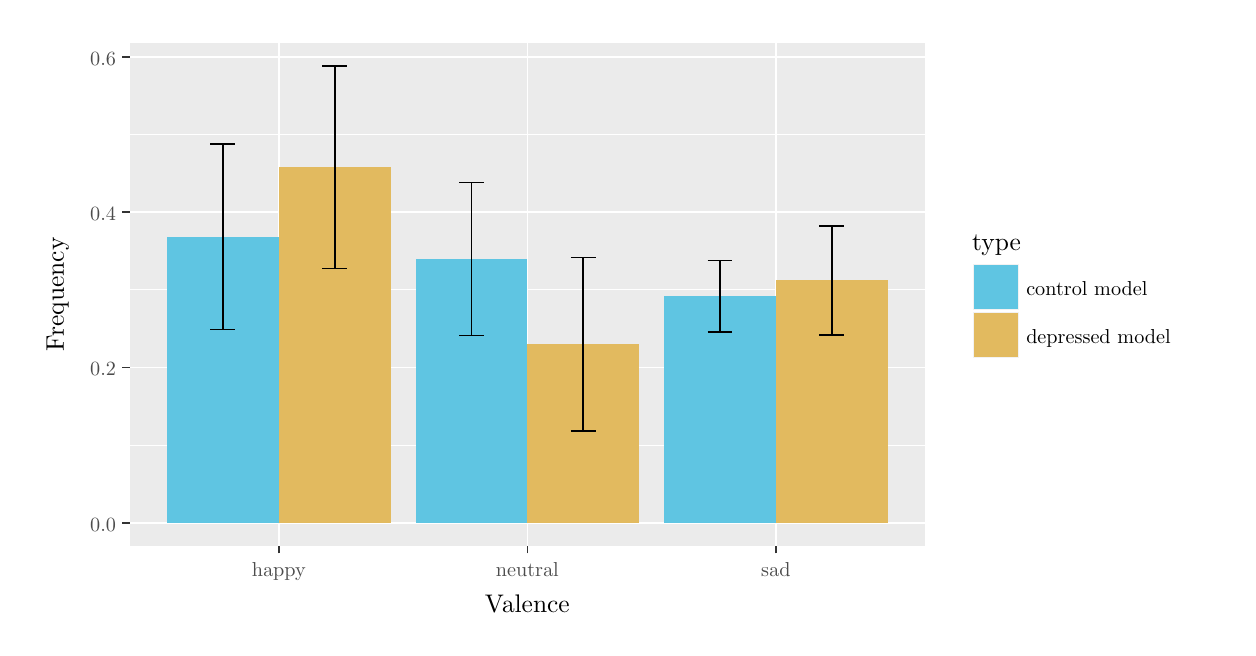
\begin{tikzpicture}[x=1pt,y=1pt]
\definecolor{fillColor}{RGB}{255,255,255}
\path[use as bounding box,fill=fillColor,fill opacity=0.00] (0,0) rectangle (433.62,216.81);
\begin{scope}
\path[clip] (  0.00,  0.00) rectangle (433.62,216.81);
\definecolor{drawColor}{RGB}{255,255,255}
\definecolor{fillColor}{RGB}{255,255,255}

\path[draw=drawColor,line width= 0.6pt,line join=round,line cap=round,fill=fillColor] ( -0.00,  0.00) rectangle (433.62,216.81);
\end{scope}
\begin{scope}
\path[clip] ( 36.87, 29.59) rectangle (324.25,211.31);
\definecolor{fillColor}{gray}{0.92}

\path[fill=fillColor] ( 36.87, 29.59) rectangle (324.25,211.31);
\definecolor{drawColor}{RGB}{255,255,255}

\path[draw=drawColor,line width= 0.3pt,line join=round] ( 36.87, 65.92) --
	(324.25, 65.92);

\path[draw=drawColor,line width= 0.3pt,line join=round] ( 36.87,122.07) --
	(324.25,122.07);

\path[draw=drawColor,line width= 0.3pt,line join=round] ( 36.87,178.21) --
	(324.25,178.21);

\path[draw=drawColor,line width= 0.6pt,line join=round] ( 36.87, 37.85) --
	(324.25, 37.85);

\path[draw=drawColor,line width= 0.6pt,line join=round] ( 36.87, 93.99) --
	(324.25, 93.99);

\path[draw=drawColor,line width= 0.6pt,line join=round] ( 36.87,150.14) --
	(324.25,150.14);

\path[draw=drawColor,line width= 0.6pt,line join=round] ( 36.87,206.28) --
	(324.25,206.28);

\path[draw=drawColor,line width= 0.6pt,line join=round] ( 90.75, 29.59) --
	( 90.75,211.31);

\path[draw=drawColor,line width= 0.6pt,line join=round] (180.56, 29.59) --
	(180.56,211.31);

\path[draw=drawColor,line width= 0.6pt,line join=round] (270.37, 29.59) --
	(270.37,211.31);
\definecolor{fillColor}{RGB}{226,186,95}

\path[fill=fillColor] ( 90.75, 37.85) rectangle (131.16,166.43);
\definecolor{fillColor}{RGB}{95,197,226}

\path[fill=fillColor] ( 50.34, 37.85) rectangle ( 90.75,141.25);
\definecolor{fillColor}{RGB}{226,186,95}

\path[fill=fillColor] (180.56, 37.85) rectangle (220.97,102.37);
\definecolor{fillColor}{RGB}{95,197,226}

\path[fill=fillColor] (140.15, 37.85) rectangle (180.56,133.23);
\definecolor{fillColor}{RGB}{226,186,95}

\path[fill=fillColor] (270.37, 37.85) rectangle (310.78,125.47);
\definecolor{fillColor}{RGB}{95,197,226}

\path[fill=fillColor] (229.95, 37.85) rectangle (270.37,119.79);
\definecolor{drawColor}{RGB}{0,0,0}

\path[draw=drawColor,line width= 0.6pt,line join=round] (106.47,203.05) --
	(115.45,203.05);

\path[draw=drawColor,line width= 0.6pt,line join=round] (110.96,203.05) --
	(110.96,129.81);

\path[draw=drawColor,line width= 0.6pt,line join=round] (106.47,129.81) --
	(115.45,129.81);

\path[draw=drawColor,line width= 0.6pt,line join=round] ( 66.05,174.76) --
	( 75.03,174.76);

\path[draw=drawColor,line width= 0.6pt,line join=round] ( 70.54,174.76) --
	( 70.54,107.73);

\path[draw=drawColor,line width= 0.6pt,line join=round] ( 66.05,107.73) --
	( 75.03,107.73);

\path[draw=drawColor,line width= 0.6pt,line join=round] (196.28,133.74) --
	(205.26,133.74);

\path[draw=drawColor,line width= 0.6pt,line join=round] (200.77,133.74) --
	(200.77, 70.99);

\path[draw=drawColor,line width= 0.6pt,line join=round] (196.28, 70.99) --
	(205.26, 70.99);

\path[draw=drawColor,line width= 0.6pt,line join=round] (155.86,160.90) --
	(164.84,160.90);

\path[draw=drawColor,line width= 0.6pt,line join=round] (160.35,160.90) --
	(160.35,105.57);

\path[draw=drawColor,line width= 0.6pt,line join=round] (155.86,105.57) --
	(164.84,105.57);

\path[draw=drawColor,line width= 0.6pt,line join=round] (286.08,145.07) --
	(295.07,145.07);

\path[draw=drawColor,line width= 0.6pt,line join=round] (290.57,145.07) --
	(290.57,105.87);

\path[draw=drawColor,line width= 0.6pt,line join=round] (286.08,105.87) --
	(295.07,105.87);

\path[draw=drawColor,line width= 0.6pt,line join=round] (245.67,132.68) --
	(254.65,132.68);

\path[draw=drawColor,line width= 0.6pt,line join=round] (250.16,132.68) --
	(250.16,106.89);

\path[draw=drawColor,line width= 0.6pt,line join=round] (245.67,106.89) --
	(254.65,106.89);
\end{scope}
\begin{scope}
\path[clip] (  0.00,  0.00) rectangle (433.62,216.81);
\definecolor{drawColor}{gray}{0.30}

\node[text=drawColor,anchor=base east,inner sep=0pt, outer sep=0pt, scale=  0.73] at ( 31.92, 34.82) {0.0};

\node[text=drawColor,anchor=base east,inner sep=0pt, outer sep=0pt, scale=  0.73] at ( 31.92, 90.96) {0.2};

\node[text=drawColor,anchor=base east,inner sep=0pt, outer sep=0pt, scale=  0.73] at ( 31.92,147.11) {0.4};

\node[text=drawColor,anchor=base east,inner sep=0pt, outer sep=0pt, scale=  0.73] at ( 31.92,203.25) {0.6};
\end{scope}
\begin{scope}
\path[clip] (  0.00,  0.00) rectangle (433.62,216.81);
\definecolor{drawColor}{gray}{0.20}

\path[draw=drawColor,line width= 0.6pt,line join=round] ( 34.12, 37.85) --
	( 36.87, 37.85);

\path[draw=drawColor,line width= 0.6pt,line join=round] ( 34.12, 93.99) --
	( 36.87, 93.99);

\path[draw=drawColor,line width= 0.6pt,line join=round] ( 34.12,150.14) --
	( 36.87,150.14);

\path[draw=drawColor,line width= 0.6pt,line join=round] ( 34.12,206.28) --
	( 36.87,206.28);
\end{scope}
\begin{scope}
\path[clip] (  0.00,  0.00) rectangle (433.62,216.81);
\definecolor{drawColor}{gray}{0.20}

\path[draw=drawColor,line width= 0.6pt,line join=round] ( 90.75, 26.84) --
	( 90.75, 29.59);

\path[draw=drawColor,line width= 0.6pt,line join=round] (180.56, 26.84) --
	(180.56, 29.59);

\path[draw=drawColor,line width= 0.6pt,line join=round] (270.37, 26.84) --
	(270.37, 29.59);
\end{scope}
\begin{scope}
\path[clip] (  0.00,  0.00) rectangle (433.62,216.81);
\definecolor{drawColor}{gray}{0.30}

\node[text=drawColor,anchor=base,inner sep=0pt, outer sep=0pt, scale=  0.73] at ( 90.75, 18.58) {happy};

\node[text=drawColor,anchor=base,inner sep=0pt, outer sep=0pt, scale=  0.73] at (180.56, 18.58) {neutral};

\node[text=drawColor,anchor=base,inner sep=0pt, outer sep=0pt, scale=  0.73] at (270.37, 18.58) {sad};
\end{scope}
\begin{scope}
\path[clip] (  0.00,  0.00) rectangle (433.62,216.81);
\definecolor{drawColor}{RGB}{0,0,0}

\node[text=drawColor,anchor=base,inner sep=0pt, outer sep=0pt, scale=  0.92] at (180.56,  5.50) {Valence};
\end{scope}
\begin{scope}
\path[clip] (  0.00,  0.00) rectangle (433.62,216.81);
\definecolor{drawColor}{RGB}{0,0,0}

\node[text=drawColor,rotate= 90.00,anchor=base,inner sep=0pt, outer sep=0pt, scale=  0.92] at ( 13.08,120.45) {Frequency};
\end{scope}
\begin{scope}
\path[clip] (  0.00,  0.00) rectangle (433.62,216.81);
\definecolor{fillColor}{RGB}{255,255,255}

\path[fill=fillColor] (335.63, 91.46) rectangle (428.12,149.44);
\end{scope}
\begin{scope}
\path[clip] (  0.00,  0.00) rectangle (433.62,216.81);
\definecolor{drawColor}{RGB}{0,0,0}

\node[text=drawColor,anchor=base west,inner sep=0pt, outer sep=0pt, scale=  0.92] at (341.32,136.17) {type};
\end{scope}
\begin{scope}
\path[clip] (  0.00,  0.00) rectangle (433.62,216.81);
\definecolor{drawColor}{RGB}{255,255,255}
\definecolor{fillColor}{gray}{0.95}

\path[draw=drawColor,line width= 0.6pt,line join=round,line cap=round,fill=fillColor] (341.32,114.49) rectangle (358.67,131.84);
\end{scope}
\begin{scope}
\path[clip] (  0.00,  0.00) rectangle (433.62,216.81);
\definecolor{fillColor}{RGB}{95,197,226}

\path[fill=fillColor] (342.04,115.20) rectangle (357.96,131.13);
\end{scope}
\begin{scope}
\path[clip] (  0.00,  0.00) rectangle (433.62,216.81);
\definecolor{drawColor}{RGB}{255,255,255}
\definecolor{fillColor}{gray}{0.95}

\path[draw=drawColor,line width= 0.6pt,line join=round,line cap=round,fill=fillColor] (341.32, 97.15) rectangle (358.67,114.49);
\end{scope}
\begin{scope}
\path[clip] (  0.00,  0.00) rectangle (433.62,216.81);
\definecolor{fillColor}{RGB}{226,186,95}

\path[fill=fillColor] (342.04, 97.86) rectangle (357.96,113.78);
\end{scope}
\begin{scope}
\path[clip] (  0.00,  0.00) rectangle (433.62,216.81);
\definecolor{drawColor}{RGB}{0,0,0}

\node[text=drawColor,anchor=base west,inner sep=0pt, outer sep=0pt, scale=  0.73] at (360.84,120.13) {control model};
\end{scope}
\begin{scope}
\path[clip] (  0.00,  0.00) rectangle (433.62,216.81);
\definecolor{drawColor}{RGB}{0,0,0}

\node[text=drawColor,anchor=base west,inner sep=0pt, outer sep=0pt, scale=  0.73] at (360.84,102.79) {depressed model};
\end{scope}
\end{tikzpicture}
